\xchapter{Experimentos}{Coleta e análise de dados}

Nesta seção irei mostrar o resultado das medições de latência realizadas no Raspberry. Será comparado os valores entre diferentes versões do kernel, entre diferentes tipos de interrupção e entre diferentes cargas na CPU.

\section{Configuração do teste}

As medições foram agrupadas por tipo de kernel, tipo de interrupção e carga na CPU, resultando em um total de 18 grupos de teste. Cada grupo passou por uma bateria de medições. Em cada bateria de teste, foram executadas 50000 medições com um intervalo de 20ms entre elas. 

O INTSight gera 2 arquivos no format CSV para cada bateria de medições. Um dos arquivos chamado name contém o tipo de evento que disparou a coleta do tempo de sistema. Outro arquivo com o nome do tipo de contador utilizado, ktime\_mono\_fast em todos os teste deste trabalho, contém o valor do contador no instante que a coleta foi disparada. Em ambos os arquivos, cada medição ocupa uma linha do arquivo.

No repositório do INTSight é disponibilizado um script em R que faz o junção destes arquivos em um único utilzando as seguintes informação: position (posição do item dentro da medição), run (número da medição dentro da bateria), name (evento que disparou a medição), ktime\_mono\_fast (valor do contador de tempo). Para consolidar os resultados das 18 baterias, foi feito um script python que encontra-se disponível em github. Este script também faz um tratamento dos dados úteis, pois o INTSight pode apresentar valores zerados quando ocorre algum erro durante uma medição.

\section{Visão geral}

A primeira letra representa o kernel testado: (R)aspberry padrão ou (P)reempt-RT.
A segunda letra é o tipo de interrupção testado: (S)oftirq, (T)asklet ou (W)orkqueue.
O terceiro caracter é a carga na cpu: 0 thread, 1 thread, (M)any threads (256).

Na tabela \ref{table:rpi} temos uma visão sumarizada do tempo de latência em nanossegundos de todos os testes realizados com o kernel padrão enquanto na tabela \ref{table:prt} temos uma visão dos testes no Preempt-RT.

\begin{table}[h!]
\centering
\begin{center}
\begin{tabular}{|c||r|r|r|r|r|r|r|r|r|}
\toprule
Percentil &    RS0 &     RS1 &    RSM &    RT0 &    RT1 &    RTM &    RW0 &     RW1 &      RWM \\
\midrule
    min &    833 &     782 &    781 &    625 &    938 &    573 &   7604 &    5730 &     5156 \\
    25\% &   1041 &     937 &    937 &   1145 &   1145 &   1146 &   8021 &    8073 &     8750 \\
    50\% &   1042 &     938 &    938 &   1146 &   1146 &   1146 &   8124 &    8177 &     8854 \\
    75\% &   1094 &     990 &    990 &   1198 &   1198 &   1250 &   8229 &    8802 &     8958 \\
    90\% &   1146 &    1042 &   1042 &   1302 &   1302 &   1406 &   8489 &    9011 &     9218 \\
    95\% &   1198 &    1823 &   1146 &   1406 &   1927 &   2187 &  11823 &    9896 &     9791 \\
    99\% &   6041 &    5833 &   5937 &   6250 &   6251 &   6198 &  16667 &   18021 &    18282 \\
    99.9\% &   6927 &    7291 &   7083 &   7292 &   8073 &  10156 &  31615 &   27916 &    25260 \\
    max &  15156 &  191821 &  19375 &  34998 &  25834 &  45260 &  84635 &  983798 &  4153458 \\
\bottomrule
\end{tabular}
\end{center}
\caption{Principais dados das medidas do kernel padrão}
\label{table:rpi}
\end{table}

\begin{table}[h!]
\centering
\begin{center}
\begin{tabular}{|c||r|r|r|r|r|r|r|r|r|}
\toprule
Percentil &    PS0 &    PS1 &    PSM &    PT0 &    PT1 &    PTM &    PW0 &     PW1 &    PWM \\
\midrule
    min &   1197 &   1146 &   1197 &   1614 &   1563 &   1614 &  11563 &   11562 &  11562 \\
    25\% &   1406 &   1406 &   1406 &   1823 &   1823 &   1823 &  12084 &   12084 &  12083 \\
    50\% &   1407 &   1407 &   1458 &   1875 &   1875 &   1875 &  12239 &   12240 &  12187 \\
    75\% &   1459 &   1458 &   1459 &   1927 &   1927 &   1875 &  12396 &   12447 &  12344 \\
    90\% &   1510 &   1510 &   1510 &   1980 &   1979 &   1927 &  12761 &   12760 &  12656 \\
    95\% &   1511 &   1511 &   1511 &   2032 &   2031 &   1979 &  13334 &   13177 &  13073 \\
    99\% &   1979 &   1823 &   1979 &   2448 &   3073 &   3125 &  21615 &   23490 &  19323 \\
    99.9\% &   4896 &   4167 &   4844 &   5469 &   5729 &   5468 &  42188 &   44271 &  39843 \\
    max &  18698 &  17656 &  17657 &  17343 &  16979 &  17865 &  80526 &  259583 &  86198 \\
\bottomrule
\end{tabular}
\end{center}
\caption{Principais dados das medidas do Preempt-RT}
\label{table:prt}
\end{table}

% \section{Expectativas}

% Preempt-RT mais lento na médio, melhor pior caso, menos variação.

\section{Análise comparativa}

Aqui será mostrado como cada kernel se desempenhou com diferentes cargas de trabalho em cada um dos mecanismos de interrupção. Os gráficos das sessões a seguir mostram os valores da latência nos percentis de de 90\% até 99,9\%. O valor máximo foi omitido da visualização pois costumam ser picos muito distantes do valor do percentil de 99,9\%, dificultando a análise visual do comportamento dos kernels.

\subsection{Softirq}

Na figura \ref{grafico:softirq} podemos ver como ambos os kernels se comportam para o tipo de interrupção Softirq. O Preempt-RT tem uma latência mais alta nos casos médios que se mantém até aproximadamente os percentis entre 94,6\% e 97,4\%. Nessa faixa a latência do kernel padrão começa a subir enquanto o Preempt-RT se mantém estável até aproximadamente o percentil de 98,5\%. Para o pior caso, temos a tabela \ref{table:max-softirq}.

Nos casos com a CPU ociosa, o Preempt-RT apresentou um tempo pior que o kernel padrão para o pior caso, o que contraria as expectativas.

Com a CPU com 1 thread de carga, o Preempt-RT teve uma pequena redução no seu pior tempo, enquanto o kernel padrão teve um pior tempo muito mais alto em relação a CPU ociosa. Aqui podemos ver que o kernel de tempo real consegui cumprir a sua premissa de ter um pior caso dentro de um nível aceitável, enquanto o kernel padrão não tem nenhum compromisso com o pior caso.

Com a CPU super carregada, o kernel padrão tem uma queda substancial na latência máxima, com valores próximos ao nível da CPU ociosa. O Preempt-RT teve um valor máximo semelhante ao caso com apenas 1 thread de carga.

O Preempt-RT se mostra bem estável, independente do tipo de carga na CPU, para as interrupções do tipo Softirq. O kernel padrão tem comportamento parecido com a CPU ociosa ou com a CPU sobrecarregada, mas quando possui uma carga leve, os tempos tendem a ser mais altos.

\begin{figure}[H]
  \centering
        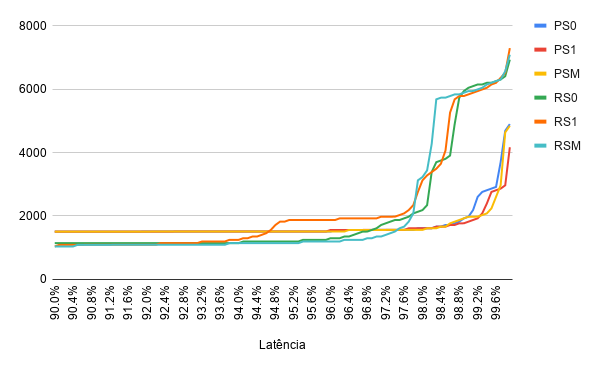
\includegraphics[width=\textwidth]{graficos/softirq.png}
        \caption{Latência com Softirq em nanossegundos}
        \label{grafico:softirq}
\end{figure}

\begin{table}[H]
\centering
\begin{center}
\begin{tabular}{|r|r|r|r|r|r|}
\toprule
    PS0 &    PS1 &    PSM &    RS0 &     RS1 &    RSM \\
\midrule
    18698 &	17656 &	17657 & 15156 & 191821 &	19375 \\
\bottomrule
\end{tabular}
\end{center}
\caption{Latência máxima para o Softirq}
\label{table:max-softirq}
\end{table}

\subsection{Tasklet}

\begin{figure}[H]
  \centering
        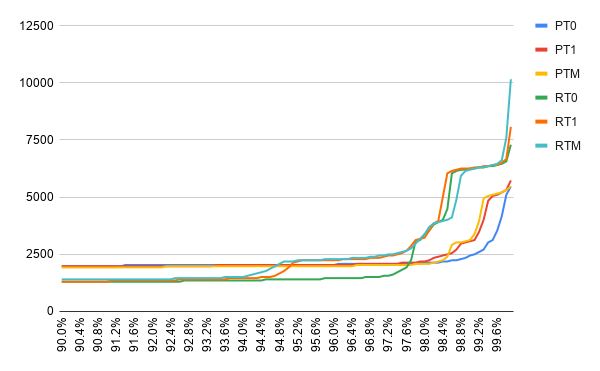
\includegraphics[width=\textwidth]{graficos/tasklet.png}
        \caption{Latência com Tasklet em nanossegundos}
        \label{grafico:tasklet}
\end{figure}

\begin{table}[H]
\centering
\begin{center}
\begin{tabular}{|r|r|r|r|r|r|}
\toprule
    PT0 &    PT1 &    PTM &    RT0 &     RT1 &    RTM \\
\midrule
    17343 &	16979 &	17865 & 34998 &	25834 &	45260 \\
\bottomrule
\end{tabular}
\end{center}
\caption{Latência máxima para o Softirq}
\label{table:max-softirq}
\end{table}

\subsection{Workqueue}

\begin{figure}[H]
  \centering
        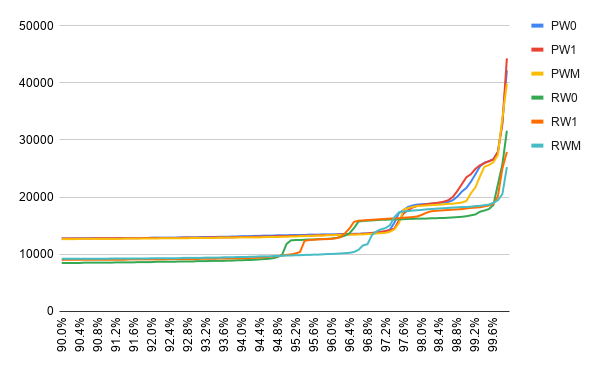
\includegraphics[width=\textwidth]{graficos/workqueue.png}
        \caption{Latência com Workqueue em nanossegundos}
        \label{grafico:workqueue}
\end{figure}

\begin{table}[H]
\centering
\begin{center}
\begin{tabular}{|r|r|r|r|r|r|}
\toprule
    PW0 &    PSW &    PWM &    RW0 &     RW1 &    RWM \\
\midrule
    80526 &	259583 &	86198 & 84635 &	983798 	4153458 \\
\bottomrule
\end{tabular}
\end{center}
\caption{Latência máxima para o Softirq}
\label{table:max-softirq}
\end{table}
